\section{Validation} 
\label{sec:validation}

This section presents, an initial simulation which was used to validate the OPNET node and process models. 

%_________________________________________________________________
%________________________SCENARIO 1_______________________________
\subsection{Scenario Topology and Details}
\label{sec:scenario1}

The network model is shown in figure \ref{fig:scenario1}.
It is used to ensure the ferry receives updates from source nodes as it passes by them and transmits them to the gateway. 
There is one gateway node, one ferry node, and seven source nodes. 
The size of the map is 0.75 km x 0.75 km with source nodes placed evenly apart by 0.375 km. 
The gateway node is at the top left corner, and the ferry is in motion indicated next to the red arrow.
The speed of the ferry is constant at 60 kmph, as it moves clockwise two times along the rectangular path that is highlighted in white.  
The simulated time was six minutes.

\begin{figure}[ht]
    \centering
    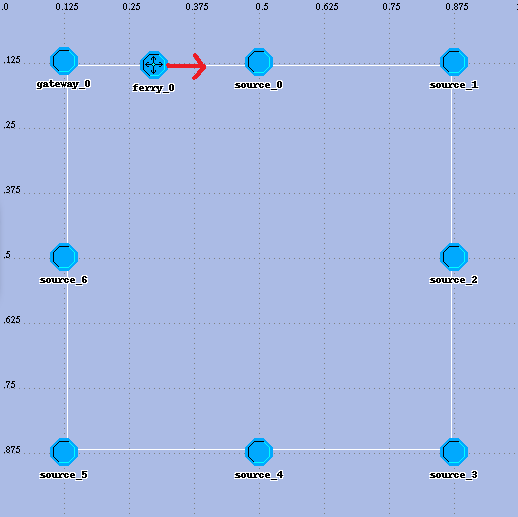
\includegraphics[width=.7\textwidth]{images/scenario1-top1r.png}
    \caption{Network Model - Validation Simulation}
    \label{fig:scenario1}
\end{figure}

\subsection{Validation Simulation Results}
\label{sec:results-validate}

A statistic measuring the number of updates received per second was created and set to be collected for the ferry and gateway nodes.
The simulation was run and the results for the ferry are shown in figure \ref{fig:result1-a}.  
From it, we can see that the ferry is receiving updates each time it passes by a source node. 

\begin{figure}[ht]
    \centering
    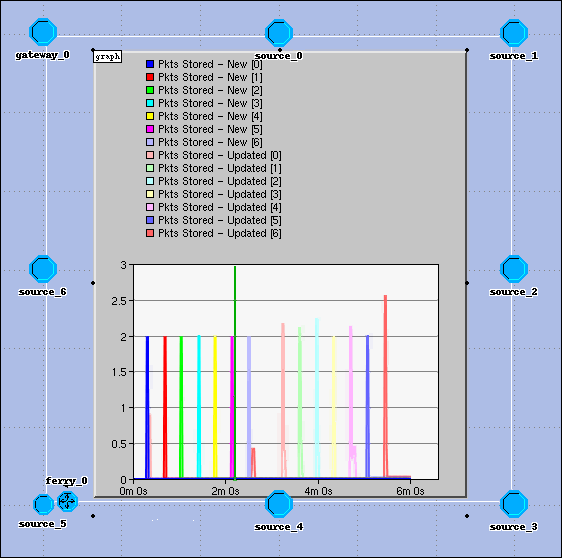
\includegraphics[width=.5\textwidth]{images/scenario1-result-received.png}
    \caption{Update Packets Received by the Ferry Node}
    \label{fig:result1-a}
\end{figure}

Results collected for the gateway may be seen in \ref{fig:result1-b}.
From the figure, it is clear that there are two spikes in the graph which corresponds to the ferry transmitting the updates it has collected. 
The ferry node traverses its path twice in this simulation which is why there are two spikes.
Each source node sends three update packets to the ferry node as it passes.  
Since there are seven source nodes, this accounts for the 21 packets received by the gateway node, which can be seen in figure \ref{fig:result1-b}.

\begin{figure}[ht]
    \centering
    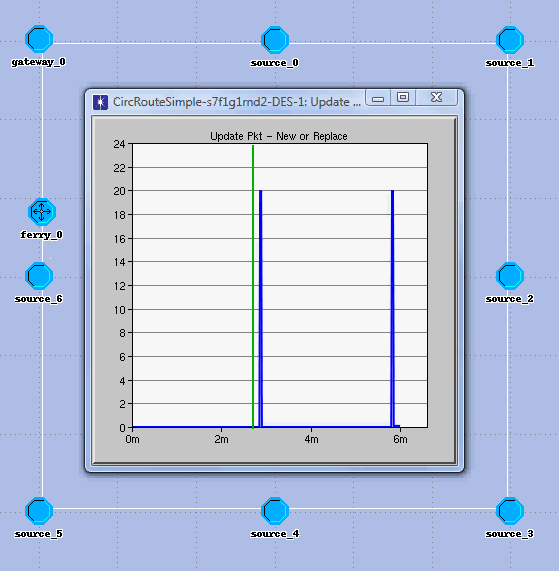
\includegraphics[width=.5\textwidth]{images/scenario1-result-gateway.png}
    \caption{Gateway receives the packet as the ferry node passes by its range of transmission}
    \label{fig:result1-b}
\end{figure}

